%!TEX root = ../main.tex

\chapter{Confocal Setup}	\label{ch::confocal_setup}
\chaptermark{Confocal Setup}

	The key measurements of this thesis are fluorescence measurements of \sivs in nanodiamonds.
	For this aim, a home-built confocal setup is used, which is described in this chapter.

	The confocal setup serves to perform a series of measurements on \fl: scanning the sample to find \sivs, recording luminescence spectra of the aforementioned, determine the saturation count rate \todo{saturation already introduced?}, and determine whether the emitter in question is a single emitter by performing photon autocorrelation measurements.
	The two key components for these measurements are 

	\begin{itemize}
		\item A Hanbury-Brown and Twiss setup to investigate the single photon character. It is built up of two avalanche photo diodes (APDs) which also serve to scan the sample in order to find emitters on the sample surface; and to perform saturation measurements.
		\item A grating spectrometer to investigate the spectral properties.
	\end{itemize}


	\begin{figure}[t] %fig::confocal_setup
		\centering
		\includegraphics[width=\linewidth]{./pics/confocal_setup.eps}
		\caption{Confocal setup}
		\label{fig::confocal_setup}
	\end{figure}

	\begin{figure}[t] %fig::hbt_spectrometer
		\centering
		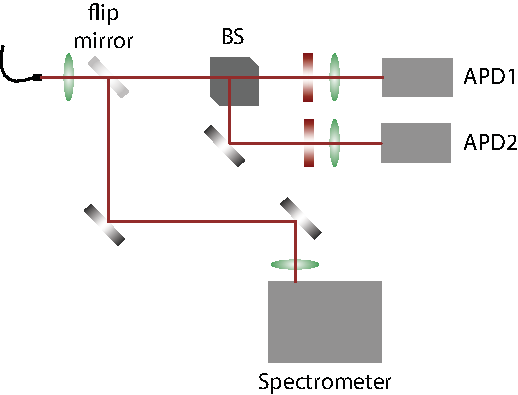
\includegraphics[width=\linewidth]{./pics/hbt_spectrometer.eps}
		\caption{HBT, spectrometer}
		\label{fig::hbt_spectrometer}
	\end{figure}

	\autoref{fig::confocal_setup} depicts a sketch of the confocal setup. 
	Except for the laser and the sample stage, the whole setup is fixed to a vertical breadboard. 
	This design allows for easy exchanging of the samples, without the need of gluing them to a vertical stage.

	The friction between the sample and the aluminum surface of the stage is sufficient that the sample does not move during scanning.
	If it is important that the sample has a a defined orientation, it is put inside of an aluminum angle.
	The stage is powered with two stepper motors (\todo{type}) in the horizontal x and y directions.
	The objective is fixed to another stage which in turn is fixed to the vertical breadboard.
	In this way, the vertical z direction is implemented for focusing the laser light on the sample.

	The bright red color at the left-hand side of the sketch represents the excitation beam path.
	The sample is excited with a continuous wave diode laser (Sch\"after-Kirchhoff, 58FCM) which emits at a wavelength of \SI{660}{\nano\meter}.
	The outlet of the light is through a pigtail fiber, the light is outcoupled and collimated exploiting an aspheric lens.
	To suppress sideband emission from the laser, a bandpass filter with a window of  \SI{10}{\nm} around a center of \SI{660}{\nm} is used.
	The excitation beam then hits a glass plate (fabricator Halle Germany \todo{thickness}) to be guided through a microscope objective and focused on the sample.
	The microscope objective is of the type Olympus, LMPlanFLN 100x and has a numerical aperture of 0.8.
	As the luminescence light from the emitter is in the same focus as the excitation laser light, it is effectively collected by the objective.
	Hence also the name confocal setup.

	The collected light then follows the detection beam path depicted in a dark red color in \autoref{fig::confocal_setup}.
	Both the excitation light reflected from the sample surface and the \fl pass through the glass plate.
	In the usual useage, the flip mirror just after the beamsplitter is lowered, allowing the light coming from the sample to move on towards a single mode fiber. 
	In front of the \smf there is a longpass filter to filter out the residual excitation light and also ambient light.
	The \fl is fed into a single-mode fiber (Thorlabs SM600) with an aspheric lens.
	The single-mode fiber serves two purpuses: First, to connect the confocal microscope with the \hbt setup and the spectrometer.
	Second, its about \SI{4.3}{\micro\meter} diameter serves as a pinhole to ensure to collect only \fl in the focal spot \todo(besser erklären).

	According to the experimental necessities, instead of the mentioned glass plate a dichroic mirror (\todo{which?}) can be employed.
	The glass plate features a high transmission of 90\%  and therefore a high collection efficiency of \fl, the dichroic mirror allows for a higher excitation intensity using the same excitation laser. 
	However, a high excitation intensity may cause permanent fluorescence intermittence of the \sivs (for further detail, refer to \todo{insert chapter}).
	In general, if a high excitation is necessary, for instance for saturation measurements \todo{saturation already introduced?}, the dichroic mirror is used; otherwise, the glass plate is used to collect as much \fl as possible.

	Another feature of the setup is that it is possible to have a look at the sample surface before starting the fluorescence measurements.
	For this purpose, the sample is illuminated with white light from a halogen lamp and the flip mirror after the glass plate is brought into an upright position to guide the light onto a CCD camera (\todo{specs}).

	As mentioned before, the \fl is either investigated with a grating spectrometer or an \hbt setup.
	The spectrometer is a Princeton Instruments Acton2500i \todo{?} spectrometer and features three gratings: 600 grooves/mm, 1200g/mm, 1800 g/mm \todo{right dimension?}.



